%%%%%%%%%%%%%%%%%%%%%%%%%%%%%%%%%%%%%%%%%%%%%%%%%%%%%%%%%%%%%%%%%%%%%%
% Lớp 12 | Ứng dụng đạo hàm để khảo sát hàm số | Cực trị của hàm số
% Dạng 2D1?2-1: Tìm cực trị của hàm số cho bởi công thức
% Số câu: 46  (sinh tự động bởi tach_cau.py; từ nay thầy sửa trực tiếp file này)
%%%%%%%%%%%%%%%%%%%%%%%%%%%%%%%%%%%%%%%%%%%%%%%%%%%%%%%%%%%%%%%%%%%%%%

%%%%%%%%%%%%%%%% TRẮC NGHIỆM 4 PHƯƠNG ÁN %%%%%%%%%%%%%%%%

% nguồn: Phan1_Lop_12_Dai_so_Chuong_1
\begin{ex}%[2D1N2-1]%[ma:aa36e913]
	Cho hàm số $f(x)$ có đạo hàm $f'(x)=(x-1)(2-x)$, $\forall x \in \mathbb{R}$. Điểm  cực đại của hàm số là
	 \choice
		{$x=1$} 
		 {$x=-2$}
		{\True  $x=2$}
		{$x=-1$} 
	\loigiai{ 
		Xét $f'(x)=0 \Leftrightarrow (x-1)(2-x)=0 \Leftrightarrow \hoac{&x=1\\&x=2.}$\\ 
		Bảng  biến thiên
		\begin{center}
			\begin{tikzpicture}[>=stealth,scale=0.8]
				 \tkzTabInit[lgt=2,espcl=2.7]
					 {$x$/0.8,$f^{\prime}
					 (x)$/0.8,$f (x)$/3}
					{$-\infty$,$1$,$2$,$+\infty$} 
				 \tkzTabLine{,-,0,+,0,-,}
				\path 
					(N12)  node[shift={(0,-0.3)}](A){$ $}
					 (N23) node[shift={(0,0.3)}](B){$ $}
					(N32) node[shift={(0,-0.3)}](C){$ $} 
					(N43) node[shift={(0,0.3)}](D){$  $};
				\foreach\X/\Y  in{A/B,B/C,C/D}\draw[->](\X)--(\Y);
			\end{tikzpicture}
		\end{center}
		Từ bảng biến thiên, suy ra hàm số  đạt cực đại tại $x=2$.
	} 
\end{ex}

% nguồn: Phan1_Lop_12_Dai_so_Chuong_1
\begin{ex}%[2D1N2-1]%[ma:3d187ea3]
	Hàm số $y=-x^3+2x^2+4x$ đạt cực trị tại hai điểm $x_1,x_2$. Khi đó giá trị của biểu thức $S=x_1^2+x_2^2$ bằng 
	 \choice
		{$\dfrac{10}{9}$} 
		 {\True $\dfrac{40}{9}$}
		 {$\dfrac{10}{3}$}
		 {$\dfrac{20}{3}$}
	 \loigiai{
		Tập xác định $\mathscr{D} =  \mathbb{R}$.\\
		Đạo hàm $y' = -3x^2+4x+4 = 0  \Leftrightarrow \hoac{&x=2\\&x=-\dfrac{2}{3}.}$\\
		Đây là hai nghiệm đơn cũng là hai cực  trị.\\
		Suy  ra $S = 2^2 + \left(-\dfrac{2}{3}\right)^2 = \dfrac{40}{9}.$
	} 
\end{ex}

% nguồn: Phan1_Lop_12_Dai_so_Chuong_1
\begin{ex}%[2D1N2-1]%[ma:cb9414eb]
	Hàm số $y=f(x)$ có đạo hàm là $f'(x) = x^2(x+1)^2(2x-1)$. Số điểm cực trị của  hàm số $y=f(x)$ là
	\choice 
		 {$3$}
		 {$0$}
		 {\True $1$}
		{$2$} 
	 \loigiai{
		Ta  có $f'(x)=0 \Leftrightarrow x^2(x+1)^2(2x-1)=0 \Leftrightarrow \hoac{&x=0\\&x=-1\\&x=\dfrac{1}{2}.}$\\
		Nhận thấy $x^2>0$, $\forall x \neq 0 \Rightarrow f'(x)$ không đổi dấu khi qua nghiệm $x=0$ nên $x=0$ không phải là điểm cực trị hàm  số.\\
		Tương tự $(x+1)^2>0$, $\forall x \neq -1 \Rightarrow f'(x)$  không đổi dấu khi qua nghiệm $x=-1$ nên $x=-1$ không phải là điểm cực trị hàm số.\\
		$f'(x)$ cùng dấu với nhị thức $2x-1$  nên $x=\dfrac{1}{2}$ là điểm cực trị của hàm số.
	} 
\end{ex}

% nguồn: Phan1_Lop_12_Dai_so_Chuong_1
\begin{ex}%[2D1N2-1]%[ma:7cccb009]
	Cho hàm số $f(x)$ có đạo hàm $f'(x) =  x-1$, $\forall x \in \mathbb{R}$. Hỏi $f(x)$ có bao nhiêu điểm cực trị?
	\choice 
		{$0$} 
		 {\True $1$}
		{$2$} 
		{$3$} 
	 \loigiai{
		Ta có $f'(x)=0 \Leftrightarrow x-1=0 \Leftrightarrow x=1$, suy ra $f'(x)$ đổi dấu một lần khi  $x$ đi qua giá trị $x=1$ nên hàm số $f(x)$ có $1$ điểm cực trị.
	} 
\end{ex}

% nguồn: Phan1_Lop_12_Dai_so_Chuong_1
\begin{ex}%[2D1N2-1]%[ma:46bb5f69]
	Cho hàm số $y=x^3-3x^2+2$. Điểm cực  tiểu của đồ thị hàm số có tọa độ là
	\choice 
		{$(2;2)$} 
		{$(2;-2)$} 
		{$(0;-2)$} 
		 {\True $(0;2)$}
	 \loigiai{
		Ta  có $y'=3x^2-6x$; $y''=6x-6$. Xét $y'=0 \Leftrightarrow \hoac{&x=0\\&x=2.}$\\
		 Ta thấy $y''(0)=-6<0 \Rightarrow$ Hàm số có điểm cực tiểu $x=0$.\\
		Vậy tọa độ điểm cực tiểu của đồ thị hàm số là $(0;2)$. 
	} 
\end{ex}

% nguồn: Phan1_Lop_12_Dai_so_Chuong_1
\begin{ex}%[2D1N2-1]%[ma:7d04e29f]
	Tìm giá trị cực tiểu của  hàm số $y=-x^3+3x+4$.
	 \choice
		{\True $y_{CT}  = 2$}
		 {$y_{CT} = 1$}
		 {$y_{CT} = 6$}
		{$y_{CT} = -1$} 
	\loigiai{ 
		Tập xác định của hàm số  $\mathscr{D} = \mathbb{R}$.\\
		Ta có $y'=-3x^2+3$, $y'=0  \Leftrightarrow -3x^2+3=0 \Leftrightarrow \hoac{&x=-1 \Rightarrow y=2\\&x=1 \Rightarrow y=6.}$\\
		 Bảng biến thiên
		\begin{center}
			\begin{tikzpicture}[>=stealth,scale=0.8]
				 \tkzTabInit[lgt=2,espcl=2.7]
					 {$x$/0.8,$y^{\prime}$/0.8,$y$/3}
					{$-\infty$,$-1$,$1$,$+\infty$} 
				\tkzTabLine{,-,0,+,0,-,} 
				 \path
					 (N12) node[shift={(0,-0.3)}](A){$+\infty$}
					 (N23) node[shift={(0,0.3)}](B){$2$}
					(N32)  node[shift={(0,-0.3)}](C){$6$}
					(N43) node[shift={(0,0.3)}](D){$-\infty$}; 
				\foreach\X/\Y  in{A/B,B/C,C/D}\draw[->](\X)--(\Y);
			\end{tikzpicture}
		\end{center}
		Vậy giá trị cực tiểu của hàm số $y_{CT} = 2$  tại $x=-1$.
	 }
\end{ex}

% nguồn: Phan1_Lop_12_Dai_so_Chuong_1
\begin{ex}%[2D1N2-1]%[ma:4ac9ce1e]
	Tổng hai giá trị cực trị của hàm  số $y=\dfrac{2x^2-x+1}{1-x}$ bằng
	\choice 
		 {$5$}
		 {$-4$}
		{\True $-6$} 
		 {$7$}
	 \loigiai{
		Ta  có $y' = \dfrac{-2x^2+4x}{(1-x)^2} = 0 \Leftrightarrow \hoac{&x=0&\Rightarrow& y = 1\\&x=2&\Rightarrow& y = -7.}$\\
		Tổng của hai giá  trị cực trị là $1+(-7)=-6$.
	} 
\end{ex}

% nguồn: Phan1_Lop_12_Dai_so_Chuong_1
\begin{ex}%[2D1N2-1]%[ma:0c2d4894]
	Cho hàm số $y=f(x)$ liên tục trên $\mathbb{R}$ và có $f'(x)=(x-1)^2(x^2-5x+6)$. Số điểm cực trị  của hàm số đã cho là
	 \choice
		{$5$} 
		{$3$} 
		{\True  $2$}
		{$4$} 
	\loigiai{ 
		Ta có $f'(x)=(x-1)^2(x^2-5x+6)  = (x-1)^2(x-2)(x-3)$.\\
		Do $f'(x)=0$ có $1$ nghiệm kép $x=1$ và hai nghiệm đơn $x=2$, $x=3$ nên $f'(x)$ đổi dấu hai lần qua $x=2$ và $x=3$. Do  đó hàm số có $2$ điểm cực trị.
	} 
\end{ex}

% nguồn: Phan1_Lop_12_Dai_so_Chuong_1
\begin{ex}%[2D1H2-1]%[ma:29b32657]
	Cho hàm số $y=7x^3+9x^2-3x-4$. Khẳng định nào sau đây là \textbf{sai}? 
	 \choice
		{Giá trị  cực đại $y=1$}
		{Hàm  số đạt cực tiểu tại $x=\dfrac{1}{7}$}
		{\True Giá trị cực  tiểu $y=\dfrac{1}{7}$}
		{Hàm số  đạt cực đại tại $x=-1$}
	\loigiai{ 
		Tập xác định $\mathbb{R}$.\\ 
		 $y'=21x^2+18x-3$.\\
		$y'=0 \Leftrightarrow x=-1 \text{ hoặc } x=\dfrac{1}{7}$.\\ 
		Do đó, hàm số đạt cực  đại tại $x=-1, y_{\text{ CĐ}}=1$.\\
		 Hàm số đạt cực tiểu tại $x=\dfrac{1}{7}, y_{\text{ CT}}=- \dfrac{207}{49}$.
	 }
\end{ex}

% nguồn: Phan1_Lop_12_Dai_so_Chuong_1
\begin{ex}%[2D1H2-1]%[ma:728467e1]
	Nếu hàm số $y=f(x)$ có đạo hàm $f'(x)=6-\dfrac{1}{\sqrt {x^2 + 1}},\forall \in \mathbb{R}$ thì giá trị nhỏ nhất của hàm số  trên đoạn $[4;6]$ bằng
	\choice 
		{\True $f(4)$} 
		 {$f(6)$}
		{$f(5)$} 
		 {$f(\sqrt {24})$}
	\loigiai{ 
		Ta  có
		\begin{eqnarray*}
			&&f'(x)=0 \Leftrightarrow \dfrac{1}{\sqrt  {x^2+1}}=6\\
			 &\Leftrightarrow& \sqrt{x^2+1}=\dfrac{1}{6}\Leftrightarrow x^2-\dfrac{35}{36} = 0\\
			&\Leftrightarrow& \hoac{&x=-\dfrac{\sqrt  {35}}{6} \notin [4;6]\\&x=\dfrac{\sqrt {35}}{6} \notin [4;6].}
		\end{eqnarray*}
		Ta có $f'(x)>0,\forall x \in [4;6]$, nên hàm số  đồng biến trên $[4;6]$.\\
		Vậy giá trị nhỏ nhất của hàm số là  $f(4)$.
	 }
\end{ex}

% nguồn: Phan1_Lop_12_Dai_so_Chuong_1
\begin{ex}%[2D1H2-1]%[ma:a4cac9a3]
	Cho hàm số $y=f(x)$ có đạo hàm trên $\mathbb{R}$ và có bảng xét  dấu của đạo hàm như sau
	\begin{center}
		\begin{tikzpicture}
			 \tkzTabInit[nocadre,lgt=1.2,espcl=2.0]
				{$x$ /1,$f'(x)$ /1} 
				 {$-\infty$,$8$,$11$,$12$,$+\infty$}
			 \tkzTabLine{,+,0,-,0,+,0,-,}
		\end{tikzpicture}
	\end{center}
	Giá trị nhỏ nhất của hàm số $y=f(x)$  trên đoạn $[8;12]$ bằng
	 \choice
		{$f(8)$} 
		{$f(10)$} 
		 {\True $f(11)$}
		 {$f(12)$}
	 \loigiai{
		 Ta có bảng biến thiên của hàm số như sau
		\begin{center}
			\begin{tikzpicture}
				 \tkzTabInit[nocadre,lgt=1.2,espcl=2.0]
					{$x$  /1,$f'(x)$ /1,$f (x)$/2}
					{$-\infty$,$8$,$11$,$12$,$+\infty$} 
				\tkzTabLine{,+,0,-,0,+,0,-,} 
				\tkzTabVar{-/,+/$f (8)$,-/$f (11)$,+/$f  (12)$,-/}
			\end{tikzpicture}
		\end{center}
		Vậy, giá trị nhỏ nhất của hàm  số $y=f(x)$ trên đoạn $[8;12]$ bằng $f(11)$.
	} 
\end{ex}

% nguồn: Phan1_Lop_12_Dai_so_Chuong_1
\begin{ex}%[2D1H2-1]%[ma:6ffd7e14]
	\immini{Cho hàm số $y=f(x)$ có  đồ thị đạo hàm $f'(x)$ như hình bên. Giá trị lớn nhất của hàm số $y=f(x)$ trên đoạn $[-1; 2]$ bằng
	 \choice
		{$f(-1)$} 
		 {$f(0)$}
		{\True  $f(1)$}
		{$f(2)$}} 
		{\resizebox{!}{5cm}{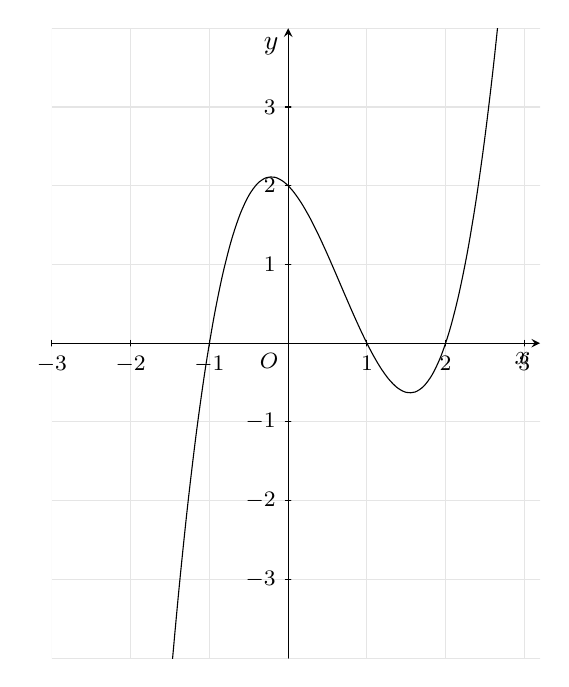
\begin{tikzpicture}[line join=round,line cap=round,>=stealth]
		\begin{scope}
			\clip (-3,-4)  rectangle (3.2,4);
			 \draw[gray!20](-4,-4) grid (4,4);
			\draw[samples=100,domain=-5.5:5.5,smooth,variable=\x] 
				 plot (\x,{(\x)^3+-2*(\x)^2+-(\x)+2});
		\end{scope}
		 \draw[->] (-3,0)--(3.2,0) node[below left] {$x$};
		 \draw[->] (0,-4)--(0,4) node[below left] {$y$};
		\draw (0,0) node  [below left] {\footnotesize $O$};
		\foreach \x  in {-3,-2,-1,1,2,3}
		\draw[thin] (\x,1pt)--(\x,-1pt) node [below]  {\footnotesize $\x$};
		\foreach \y in {-3,-2,-1,1,2,3} 
		\draw[thin] (1pt,\y)--(-1pt,\y) node [left] {\footnotesize  $\y$};
	\end{tikzpicture}
		}} 
	 \loigiai{
		Ta  có: $f'(x)=0\Leftrightarrow \hoac{&x=-1\\&x=1\\&x=2.}$\\
		Bảng  biên thiên
		\begin{center}
			
\begin{tikzpicture}
				 \tkzTabInit[nocadre,lgt=1,espcl=2]
					{$x$ /1,$y'$ /1,$y$ /2} 
					{$-\infty$,$-1$,$1$,$2$,$+\infty$} 
				 \tkzTabLine{,-,0,+,0,-,0,+}
				\tkzTabVar{+/$+\infty$,-/$f (-1)$,+/$f  (1)$,-/$f (2)$,+/$+\infty$}
			\end{tikzpicture}
		\end{center}
		 Dựa vào bảng biến thiên trên đoạn $[-1;2]$ hàm số có giá trị lớn nhất là $f(1)$.
	 }
\end{ex}

% nguồn: Phan1_Lop_12_Dai_so_Chuong_1
\begin{ex}%[2D1H2-1]%[ma:33cc84fa]
	Cho hàm số $f(x)=x\mathrm{e}^x$. Khẳng  định nào sau đây là \textbf{đúng}?
	\choice 
		{$x=1$ là  điểm cực đại của hàm số}
		{$x=-1$ là điểm cực đại  của hàm số}
		{$x=1$ là điểm cực tiểu của hàm số} 
		{\True $x=-1$ là điểm cực tiểu  của hàm số}
	\loigiai{ 
		Ta có: $f'(x)=\mathrm{e}^x\left(x+1\right)$ , $f'(x)=0$ $\Leftrightarrow $ $x=-1$.\\ 
		Bảng  xét dấu của đạo hàm:
		\begin{center}
			
\begin{tikzpicture}
				\tkzTabInit[nocadre,espcl=3,lgt=1.5] 
					 {$x$/0.7,$y'$/0.7,$y$/2.1}
					 {$-\infty$,$-1$,$+\infty$}
				\tkzTabLine{,-,0,+} 
				\tkzTabVar{+/$0$,-/$\dfrac{-1}{\mathrm{e}}$,+/$+\infty$} 
			\end{tikzpicture}
		\end{center}
	Từ đó, hàm số đạt cực tiểu tại $x=-1$.} 
\end{ex}

% nguồn: Phan1_Lop_12_Dai_so_Chuong_1
\begin{ex}%[2D1H2-1]%[ma:46261b45]
	Cho hàm số $y=f(x)$ có đạo hàm $f'(x)=2(x^2-1)(x+2)$, $\forall\mathbb{R}$. Hàm số có bao nhiêu  điểm cực tiểu?
	Số điểm cực trị của hàm số  đã cho là
	 \choice
		 {\True $2$}
		 {$0$}
		{$3$} 
		 {$1$}
	 \loigiai{
		 Ta có $f'(x)=2(x^2-1)(x+2)=0\Leftrightarrow \hoac{&x=1\\&x=-1\\&x=2}$.\\
		Bảng xét dấu 
		\begin{center}
			\begin{tikzpicture}
				 \tkzTabInit[lgt=1,espcl=3]
					{$x$/0.7,$f'(x)$/0.7} 
					 {$-\infty$,$-2$,$-1$,$1$,$+\infty$}
				\tkzTabLine{,-,0,+,0,-,0,+,} 
			\end{tikzpicture}
		\end{center}
		 Suy ra hàm số đã cho có hai cực tiểu là $x=-2$, $x=1$.
	 }
\end{ex}

% nguồn: Phan1_Lop_12_Dai_so_Chuong_1
\begin{ex}%[2D1V2-1]%[ma:c365f478]
	Nếu hàm số $y=f(x)$ có đạo hàm $f'(x)=-\sin x\cdot \cos x-\dfrac{1}{\sqrt{2}}, \forall x \in  \mathbb{R}$ thỉ giá trị lớn nhất của hàm số trên đoạn $[4; 6]$ là
	 \choice
		{\True  $f(4)$}
		 {$f(6)$}
		{$f(5)$} 
		{$f(\sqrt{24})$} 
	 \loigiai{
		Ta  có $f'( x) = 0 \Leftrightarrow \sin 2x=-\sqrt 2$ (Phương trình vô nghiệm).\\
		Ta có $f'(x)  < 0,\forall x \in [4;6]$, nên hàm số nghịch biến trên đoạn $[4;6]$.\\
		Vậy giá trị lớn nhất trên đoạn $[4;6]$ là  $f(4)$.
	} 
\end{ex}

% nguồn: Phan1_Lop_12_Dai_so_Chuong_1
\begin{ex}%[2D1V2-1]%[ma:596d9238]
	Giá trị lớn  nhất của hàm số $f(x)=3x+\sin \dfrac{x}{2}$ trền đoạn $[0; 2\pi]$ là
	 \choice
		{\True  $6\pi$}
		{$7\pi$} 
		{$8\pi$} 
		 {$9\pi$}
	\loigiai{ 
		Ta có  $f'(x)=3+\dfrac{1}{2}\cos \dfrac{x}{2}=0$ (Phương trình vô nghiệm).\\
		Do đó $f'(x)>0,\forall x  \in [0;2\pi]$, nên hàm số đồng biến trên đoạn $[0;2\pi]$.\\
		Do  đó giá trị lớn nhất là $f(2\pi)=6\pi$.
	} 
\end{ex}

% nguồn: Phan1_Lop_12_Dai_so_Chuong_1
\begin{ex}%[2D1Y2-1]%[ma:1acf5315]
	Biết rằng hàm số $ f(x)=x^2e^x+a $ ($ a $ là hằng số) có giá trị cực tiểu bằng $  1 $. Giá trị cực đại của hàm số này là
	 \choice
		{$ \dfrac{4}{e^2}  $}
		{$ \dfrac{1}{e}+1  $}
		 {\True $ \dfrac{4}{e^2}+1 $}
		 {$ 1-\dfrac{4}{e^2} $}
	 \loigiai{
		$ f'(x)=xe^x(x+2),\forall x  \in \mathbb{R} $.\\
		Bảng xét  dấu của đạo hàm:
		\begin{center}
			\begin{tikzpicture}[font=\normalsize,t style/.style={style=solid}]
				 \tkzTabInit[nocadre=true,lgt=1.2,espcl=2.5,deltacl=0.5]
					 {$x$ /0.75,$f'(x)$/0.75}
					{$ -\infty $,$  -2 $,$ 0 $,$ +\infty $}
				\tkzTabLine{,+,0,-,0,+,} 
			\end{tikzpicture}
		\end{center}
		Giá  trị cực tiểu của hàm số là $ f(0)=1 $ suy ra $ a=1 $.\\
		Giá trị cực đại của hàm số là $ f(-2)=(-2)^2 e^{-2}+1=\dfrac{4}{e^2}+1$. 
	 }
\end{ex}

% nguồn: Phan1_Lop_12_Dai_so_Chuong_1
\begin{ex}%[2D1Y2-1]%[ma:2de16507]
	Cho hàm số $ y=f(x) $ có đạo hàm $ f'(x)=x^2(x+3) $ với $  x \in \mathbb{R} $. Số điểm cực trị của hàm số đã cho là
	 \choice
		{$ 0  $}
		{\True $ 1  $}
		{$ 2  $}
		{$ 3  $}
	\loigiai{ 
		Bảng xét dấu  của đạo hàm:
		\begin{center}
			\begin{tikzpicture}[font=\normalsize,t style/.style={style=solid}]
				 \tkzTabInit[nocadre=true,lgt=1.2,espcl=2.5,deltacl=0.5]
					 {$x$ /0.75,$f'(x)$/0.75}
					{$ -\infty  $,$ -3 $,$ 0 $,$ +\infty $}
				\tkzTabLine{,-,0,+,0,+,} 
			\end{tikzpicture}
		\end{center}
		Từ đó, hàm số $ y=f(x) $ chỉ có  một điểm cực trị là $ x=-3 $.
	 }
\end{ex}

% nguồn: Phan1_Lop_12_Dai_so_Chuong_1
\begin{ex}%[2D1Y2-1]%[ma:6f2eadcf]
	Hàm số nào sau đây \textbf{không} có cực trị? 
	\choice 
		{\True $y=\dfrac{1}{x-1} -  x$}
		{$y=x^2$} 
		{$y=-x^4 + 2x^2  + 3$}
		{$y=\dfrac{1}{4}x^4 +  \dfrac{1}{2}x^2 $}
	\loigiai{ 
		 Xét hàm số $y=\dfrac{1}{x-1} - x$ với $x \neq 1$.\\
		Ta có $y'(x)=-\dfrac{1}{(x-1)^2} - 1 <  0,\, \forall x \neq 1$.\\
		Do  $y'(x)$ luôn âm, hàm số không có cực trị.
	 }
\end{ex}


%%%%%%%%%%%%%%%% ĐÚNG/SAI %%%%%%%%%%%%%%%%

% nguồn: Phan1_Lop_12_Dai_so_Chuong_1
\begin{ex}%[2D1H2-1]%[ma:754ff0d6]
	Cho hàm số  $y=f(x)$ có $f'(x)=x(x-1)(x-2)(x-3)\ldots(x-10)$, $\forall x\in\mathbb{R}$.
	\choiceTF 
		{Hàm số $f(x)$ có $10$ điểm  cực trị}
		{\True Hàm số $f(x)$ có $5$  điểm cực đại}
		 {Hàm số $f(x)$ có $5$ điểm cực tiểu}
		 {Hàm số $f(|x|)$ có $11$ điểm cực trị}
	 \loigiai{
		\begin{itemchoice}
			 \itemch
			Phương trình $f'(x)=0$ có $11$ nghiệm  phân biệt nên hàm số $f(x)$ có $11$ điểm cực trị.
			 \itemch
			Hàm số $f(x)$ là hàm đa thức và $\lim\limits_{x\rightarrow\pm\infty}f(x)=+\infty$ nên số điểm cực tiểu nhiều hơn số điểm cực đại là $1$. Mà tổng số điểm cực trị là $11$ nên số điểm cực đại  là $5$ và số điểm cực tiểu là $6$.
			\itemch 
			Hàm số $f(x)$ là hàm đa thức và $\lim\limits_{x\rightarrow\pm\infty}f(x)=+\infty$ nên số điểm cực tiểu nhiều hơn số điểm cực đại là $1$. Mà tổng số điểm cực trị là  $11$ nên số điểm cực đại là $5$ và số điểm cực tiểu là $6$.
			\itemch 
			Số điểm cực trị của hàm số $f(|x|)$ bằng $2\cdot 10+1=21$ (vì hàm số có $10$  điểm cực trị dương).
		\end{itemchoice}
	 }
\end{ex}

% nguồn: Phan1_Lop_12_Dai_so_Chuong_1
\begin{ex}%[2D1H2-1]%[ma:e0d8cc5b]
	 Cho hàm số $y = \dfrac{x^2 - 2x + 2}{x - 1}$.
	\choiceTF 
		{Đạo hàm của hàm số là  $y' = \dfrac{x^2 - 2x}{x + 1}$}
		{\True Giá trị cực đại của hàm  số bằng $-2$}
		{Điểm cực tiểu của hàm số bằng $0$} 
		{\True Phương trình đường thẳng đi qua hai  điểm cực trị của đồ thị hàm số là $y = 2x - 2$}
	 \loigiai{
		Tập xác định $\mathscr{D} = \mathbb{R} \setminus  \{1\}$. \\
		Đạo hàm $y'  = 1 - \dfrac{1}{(x - 1)^2} = \dfrac{x^2 - 2x}{(x - 1)^2}$.
		 Cho $y'=0\Leftrightarrow \hoac{&x=0 \\ &x=2.}$ \\
		Bảng biến  thiên
		\begin{center}
			
\begin{tikzpicture}[scale=1,font=\footnotesize,line join=round,line cap=round,>=stealth]
				\tkzTabInit[nocadre=false,lgt=1,espcl=2,deltacl=0.5] 
					{$x$/.7,$y'$/.7,$y$/2} 
					{$-\infty$,$0$,$1$,$2$,$+\infty$} 
				 \tkzTabLine{,+,0,-,d,-,0,+,}
				\tkzTabVar{-/$-\infty$,+/$-2$,-D+/$-\infty$/$+\infty$,-/$2$,+/$+\infty$} 
			\end{tikzpicture}
		\end{center}
		Từ đó, ta có 
		\begin{itemchoice}
			\itemch Vì $y'= \dfrac{x^2 - 2x}{(x - 1)^2}  \neq \dfrac{x^2 - 2x}{x + 1}$.
			\itemch Giá  trị cực đại của hàm số bằng $f(0)=-2$.
			\itemch Điểm cực tiểu của  hàm số bằng $x=2$.
			\itemch Đường thẳng qua hai điểm cực trị  của hàm số là
			\[y=\dfrac{\left(x^2-2x\right)'}{(x-1)'}=2x-2.\] 
		\end{itemchoice}
	} 
\end{ex}

% nguồn: Phan1_Lop_12_Dai_so_Chuong_1
\begin{ex}%[2D1H2-1]%[ma:d7ad18f5]
	 Cho hàm số $y=\sqrt{x^2+1}$
	\choiceTF 
		{Hàm số cực đại tại $x=0$} 
		{Hàm số không có cực  trị}
		{\True  Hàm số đạt cực tiểu tại $x=0$}
		{Hàm số có hai điểm cực trị} 
	\loigiai{ 
		 Xét hàm số $y=\sqrt{x^2+1}$ có tập xác định là $\mathscr{D} = \mathbb{R}$.\\
		Đạo hàm $y'=\dfrac{x}{\sqrt{x^2+1}} =0  \Leftrightarrow x=0$.\\
		Ta có bảng  biến thiên
		\begin{center}
			\begin{tikzpicture}[>=stealth,scale=0.8]
				 \tkzTabInit[lgt=2,espcl=4]
					{$x$/0.8,$y^{\prime}$/0.8,$y$/3} 
					 {$-\infty$,$0$,$+\infty$}
				 \tkzTabLine{,-,0,+,}
				 \path
					(N12) node[shift={(0,-0.3)}](A){$+\infty$} 
					(N23)  node[shift={(0,0.3)}](B){$ $}
					(N32)  node[shift={(0,-0.3)}](C){$+\infty$};
				 \foreach\X/\Y in{A/B,B/C}\draw[->](\X)--(\Y);
			\end{tikzpicture}
		\end{center}
		\begin{itemchoice}
			\itemch Hàm  số cực tiểu tại $x=0$.
			\itemch Hàm số có một  cực trị.
			\itemch Hàm  số đạt cực tiểu tại $x=0$.
			 \itemch Hàm số có một cực trị.
		\end{itemchoice}
	} 
\end{ex}

% nguồn: Phan1_Lop_12_Dai_so_Chuong_1
\begin{ex}%[2D1H2-1]%[ma:f1ac9473]
	Cho hàm số $y=-\dfrac{1}{2}x^4 + x^2 +  \dfrac{1}{2}$.
	\choiceTF 
		{Hàm số đạt  cực tiểu tại $x=0$, giá trị cực tiểu của hàm số là $y(0)=0$}
		{Hàm số đạt cực tiểu tại các điểm $x =  \pm 1$, giá trị cực tiểu của hàm số là $y(\pm 1)=1$}
		{Hàm số đạt cực đại tại các điểm $x =  \pm 1$, giá trị cực đại của hàm số là $y(\pm 1) = \dfrac{1}{2}$}
		{\True Hàm số đạt cực tiểu tại  $x=0$, giá trị cực tiểu của hàm số là $y(0)=\dfrac{1}{2}$}
	 \loigiai{
		Ta có $y'=-2x^3+2x=0  \Leftrightarrow -2x^3+2x=0 \Leftrightarrow \hoac{&x=0\\&x=1\\&x=-1.}$
		Ta có  bảng biến thiên sau
		\begin{center}
			\begin{tikzpicture}[>=stealth,scale=0.8]
				 \tkzTabInit[lgt=2,espcl=2]
					{$x$/0.8,$y^{\prime}$/0.8,$y$/3} 
					 {$-\infty$,$-1$,$0$,$1$,$+\infty$}
				 \tkzTabLine{,+,0,-,0,+,0,-}
				\path 
					(N13)  node[shift={(0,0.3)}](A){$-\infty$}
					(N22) node[shift={(0,-0.3)}](B){$1$} 
					(N33)  node[shift={(0,0.4)}](C){$\frac{1}{2}$}
					(N42)  node[shift={(0,-0.3)}](D){$1$}
					(N53)  node[shift={(0,0.3)}](E){$-\infty$};
				\foreach\X/\Y  in{A/B,B/C,C/D,D/E}\draw[->](\X)--(\Y);
			\end{tikzpicture}
		\end{center}
		\begin{itemchoice}
			\itemch Hàm số đạt  cực tiểu tại $x=0$, giá trị cực tiểu của hàm số là $y(0)=\dfrac{1}{2}$.
			\itemch Hàm số đạt cực tiểu tại $x=0$, giá  trị cực tiểu của hàm số là $y(0)=\dfrac{1}{2}$.
			 \itemch Hàm số đạt cực đại tại $x=\pm 1$, giá trị cực tiểu của hàm số là $y(\pm 1)=0$.
			\itemch Hàm số  đạt cực tiểu tại $x=0$, giá trị cực tiểu của hàm số là $y(0)=\dfrac{1}{2}$.
		\end{itemchoice}
	} 
\end{ex}

% nguồn: Phan1_Lop_12_Dai_so_Chuong_1
\begin{ex}%[2D1V2-1]%[ma:e13a238a]
	 Cho hàm số $y=\dfrac{x^2+3x+6}{x+1}$.
	\choiceTF 
		{\True Đạo hàm của hàm số là $y^{\prime}=\dfrac{x^2+2x-3}{(x+1)^2}, \forall  x \neq-1$}
		{\True  Điểm cực tiểu của đồ thị hàm số là $(1;5)$}
		{Hàm số nghịch biến trên khoảng $(-3;1)$} 
		{Tổng khoảng  cách từ các điểm cực trị của đồ thị hàm số đến trục hoành bằng $2$}
	 \loigiai{
		\begin{itemchoice}
			 \itemch
			Tập xác định $\mathscr{D}=\mathbb{R} \backslash\{-1\}$. 
			\\Đạo hàm của hàm số  là $y^{\prime}=\dfrac{x^2+2x-3}{(x+1)^2}, \forall x \neq-1$.
			\itemch  $y^{\prime}=0 \Leftrightarrow\hoac{&x=1 \\& x=-3.}$\\
			 Bảng biến thiên
			\begin{center}
				
\begin{tikzpicture}
					\tkzTabInit[nocadre=false,lgt=1.2, 
						 espcl=2.5,deltacl=0.6]
						{$x$/0.6,$y'$/0.6,$y$/2.5}{$-\infty$,$-3$,$-1$,$1$,$+\infty$} 
					 \tkzTabLine{,+,0,-,d,-,0,+,}
					 \tkzTabVar{-/$-\infty$,+/$-3$,-D+/$-\infty$/$+\infty$,-/$5$,+/$+\infty$}
				\end{tikzpicture}
			\end{center}
			Điểm cực tiểu của đồ  thị hàm số là $(1;5)$.
			 \itemch Hàm số nghịch biến trên khoảng $(-3;-1)$ và $(-1;1)$.
			\itemch Gọi hai điểm  cực trị là $A(1;5) $; $B(-3;-3)$. Khi đó $$\mathrm{d} (A , Ox)=|5|=5, \mathrm{d}(B , Ox)=|-3|=3.$$
			Tổng khoảng cách từ các điểm cực trị của đồ thị hàm số đến trục  hoành bằng $8$.
		\end{itemchoice}
	 }
\end{ex}

% nguồn: Phan1_Lop_12_Dai_so_Chuong_1
\begin{ex}%[2D1V2-1]%[ma:6b3e8088]
	Cho hàm  số $y = f(x)$ có đạo hàm $f'(x) = (x-1)(x+2)^2$ với mọi $x \in \mathbb{R}$.
	 \choiceTF
		{Phương trình $f(x) = 0$ có duy  nhất một nghiệm $x = 1$}
		{\True Hàm số $y = f(x)$ đồng biến trên khoảng $(1, +\infty)$} 
		{\True Hàm  số $y = f(x)$ có hai điểm cực trị}
		{Hàm số $y  = |f(x)|$ có ba điểm cực đại}
	\loigiai{ 
		\begin{itemchoice}
			\itemch Sai. Ta có $f'(x)=(x-1)^2(x^2-3x+2)=(x-1)^3(x-2)$.\\ 
			 $f'(x)=0 \Leftrightarrow \heva{&x=1\\&x=2.}$\\
			Vậy phương trình $f'(x)=0$  có hai nghiệm.
			\itemch  Đúng. Bảng biến thiên $y=f(x)$.
			\begin{center}
				\begin{tikzpicture}
					 \tkzTab
						 [nocadre,lgt=1.5,espcl=3]
						{$x$/1,$f’(x)$/1,$f (x)$/2.5} 
						{$-\infty$,$1$,$2$,$+\infty$} 
						{,+,0,-,0,+,} 
						 {-/,+/,-/,+/}
				\end{tikzpicture}
			\end{center}
			Dựa  vào bảng biến thiên của hàm số $y = f(x)$ ta thấy hàm số đồng biến trên các khoảng $(-\infty;1), (2;+\infty)$. \\
			Ta có $(-3;0)  \subset (-\infty;1)$ nên hàm số $f(x)$ đồng biến trên khoảng $(-3;0)$.
			\itemch Đúng. 
			Dựa vào  bảng biến thiên của hàm số $y = f(x)$ ta thấy hàm số có hai điểm cực trị.
			\itemch Sai. 
			Ta có $y = f(x^2 - 6x  + 1) \Rightarrow y' = (x^2 - 6x +1)' f'(x^2 -6x +1) = (2x -6) f'(x^2 -6x +1). $ \\
			$ y' = 0 \Leftrightarrow (2x-6) f'(x^2 -6x +1) = 0 \Leftrightarrow 
			\heva{& 2x-6 = 0 \\ & x^2 -6x +1 = 1\\&x^2 -6x +1 = 2. } 
			\Leftrightarrow \hoac{&x=3\\&x=0\\&x=6\\&x=-3+\sqrt{10}\\&x=-3-\sqrt{10}.}$\\ 
			Bảng biến thiên $y = f(x^2 -6x +1)$. 
			\begin{center}
				
\begin{tikzpicture}
					\tkzTab 
						[nocadre,lgt=1.5,espcl=2.5] 
						{$x$/1,$y'$/1,$y$/2.5} 
						{$-\infty$,$-3-\sqrt{10}$,$0$,$-3+\sqrt{10}$,$3$,$6$,$+\infty$} 
						 {,-,0,+,0,-,0,+,0,-,0,+,}
						{+/,-/,+/,-/,+/,-/,+/} 
				\end{tikzpicture}
			\end{center}
			Dựa  vào bảng biến thiên của hàm số $y=f(x^2-6x+1)$ ta thấy hàm số có hai điểm cực đại.
		\end{itemchoice}
	 }
\end{ex}


%%%%%%%%%%%%%%%% TRẢ LỜI NGẮN %%%%%%%%%%%%%%%%

% nguồn: Phan2_Lop_12_Dai_so_Chuong_1
\begin{bt}%[2D1H2-1]%[ma:34c6aeb1]
	Giá trị cực đại của hàm số $y=\dfrac{x^2+2x-2}{x+3}$ bằng  bao nhiêu?
	\shortans{-6} 
	\loigiai{ 
		 Tập xác định $\mathscr{D}=\mathbb{R}\setminus\{-3\}$.\\
		Ta  có $y'=\dfrac{(2x+2)(x+3)-\left(x^2+2x-2\right)}{(x+3)^2}=\dfrac{x^2+6x+8}{(x+3)^2}$. \\
		Suy ra  $y'=0\Leftrightarrow\hoac{&x=-4\\
		&x=-2.}$\\ 
		 Ta lập được bảng biến thiên như sau
		\begin{center}
			\begin{tikzpicture}
				 \tkzTabInit[nocadre=true,lgt=1.2,espcl=1.8,deltacl=0.4]
					{$x$/0.7,$y'$/0.7,$y$/2} 
					{$-\infty$,$-4$,$-3$,$-2$,$+\infty$} 
				 \tkzTabLine{,+,0,-,,-,0,+,}
				\path 
					(N13)  node[shift={(0,0)}](A){$-\infty$}
					 (N22) node[shift={(0,-0.4)}](B){$-6$}
					(N33)  node[shift={(-0.4,0)}](C){$-\infty$}
					(N32) node[shift={(0.4,-0.2)}](D){$+\infty$} 
					(N43) node[shift={(0,0.4)}](E){$-2$} 
					(N52)  node[shift={(0,-0.2)}](F){$+\infty$};
				\foreach\X/\Y  in{A/B,B/C,D/E,E/F}\draw[-stealth](\X)--(\Y);
				\draw[double](N31) --(N33); 
			\end{tikzpicture}
		\end{center}
		Vậy giá trị cực đại cần tìm  là $y(-4)=-6$.
	 }
\end{bt}

% nguồn: Phan2_Lop_12_Dai_so_Chuong_1
\begin{bt}%[2D1H2-1]%[ma:15d5ade3]
	Giả sử hàm số $f(x)=x^3-6 x^2+9 x-1$ đạt cực đại tại $x=a$ và đạt cực tiểu tại $x=b$. Giá trị  của biểu thức $A=2 a+b$ là bao nhiêu?
	 \shortans{5}
	 \loigiai{
		Ta có  $f'(x)=3x^2-12x+9$.\\
		Cho $f'(x)=0\Leftrightarrow 3x^2-12x+9=0\Leftrightarrow \hoac{&x=1\\ &x=3.}$\\ 
		Bảng  biến thiên.
		\begin{center}
			\begin{tikzpicture}[scale=1,font=\footnotesize]
				 \tkzTabInit[nocadre=false,lgt=1.2,espcl=2,deltacl=0.6]
					 {$x$/0.8,$f'(x)$/0.6,$f (x)$/2}
					 {$-\infty$,$1$,$3$,$+\infty$};
				\tkzTabLine{,+,$0$,-,$0$,+,}; 
				\tkzTabVar{-/$-\infty$,+/$3$,-/$-1$,+/$+\infty$}; 
			\end{tikzpicture}
		\end{center}
		Hàm số đạt cực đại  tại $x=1$.\\
		Hàm số đạt cực tiểu tại  $x=3$.\\
		Suy ra $a=1$ và $b=3$.\\ 
		 Vậy $A=2a+b=5$.
	} 
\end{bt}

% nguồn: Phan2_Lop_12_Dai_so_Chuong_1
\begin{bt}%[2D1H2-1]%[ma:e8232fb9]
	Cho hàm số $y=-x^4+2x^2+3$ có giá trị cực đại $y_\text{ CĐ}$ và giá trị cực tiểu $y_\text{ CT}$. Giá  trị $2y_\text{ CĐ}-y_\text{ CT}$ bằng bao nhiêu? (Kết quả làm tròn đến hàng đơn vị).
	 \shortans{5}
	\loigiai{ 
		Tập xác định của hàm số là  $\mathscr{D}=\mathbb{R}$.\\
		Ta  có $y'=-4x^3+4x; y'=0\Leftrightarrow\hoac{&x=-1\\
		&x=0\\ 
		 &x=1.}$\\
		Bảng biến  thiên.
		\begin{center}
			
\begin{tikzpicture}[scale=0.9,font=\footnotesize,line join=round,line cap=round,>=stealth]
				\tkzTabInit 
					{$x$/1,$y'  $/1,$y$/3}
					{$-\infty$,$-1$,$0$,$1$,$+\infty$} 
				\tkzTabLine{,+,0,-,0,+,0,-,} 
				\tkzTabVar{-/$-\infty$,+/$4$,-/$3$,+/$4$,-/$-\infty$} 
			\end{tikzpicture}
		\end{center}
		Hàm số  đạt cực tiểu tại $x=0$ và $y_\text{ CT}=y(0)=3$.\\
		Hàm số đạt cực đại tại $x=\pm 1$ và  $y_\text{ CĐ}=y(\pm 1)=4$.\\
		 Vậy $2y_\text{ CĐ}-y_\text{ CT}=5$.
	 }
\end{bt}

% nguồn: Phan2_Lop_12_Dai_so_Chuong_1
\begin{bt}%[2D1H2-1]%[ma:54b37f65]
	Đồ thị hàm số $y=x^3-3x^2-9x+1$ có hai  điểm cực trị là $A$ và $B$. Tính khoảng cách từ gốc tọa độ $O$ đến đường thẳng $AB$ (làm tròn đến hàng phần trăm).
	\shortans{0,25} 
	\loigiai{ 
		Hàm số $y=x^3-3x^2-9x+1$ có $y' = 3x^2-6x-9 =0  \Leftrightarrow \hoac{&x=-1 \rightarrow y = 6\\&x=3 \rightarrow y = -26.}$\\
		Hàm số hai điểm cực trị là  $A(-1;16)$ và $B(3;-26)$.\\
		Phương trình  đường thẳng qua $AB$ là $8x+y+2=0$.\\
		Khi đó khoảng cách từ $O(0;0)$  đến $AB$ là
		\[ 
		\mathrm{d}(O;AB)  = \dfrac{|8 \cdot 0 + 0 +2|}{\sqrt{8^2+1^2}} = \dfrac{2}{\sqrt{65}} \approx 0{,}25.
		\] 
	} 
\end{bt}

% nguồn: Phan2_Lop_12_Dai_so_Chuong_1
\begin{bt}%[2D1H2-1]%[ma:ef1a38d1]
	Cho hàm số $y=f(x)$ thỏa mãn $f'(x)=(x-1)(x-2)^2(x-3)$. Tổng các điểm cực  trị của hàm số $y=f(x)$ là bao nhiêu?
	\shortans{4} 
	\loigiai{ 
		Ta có $f'(x)=0 \Leftrightarrow (x-1)(x-2)^2(x-3)=0 \Leftrightarrow \hoac{&x=1\\&x=2 \quad\text{ (nghiệm bội chẵn)}\\&x=3.}$\\ 
		Bảng xét  dấu
		\begin{center}
			\begin{tikzpicture}
				\tkzTabInit[nocadre,lgt=2,espcl=2,deltacl=0.5] 
					{$x$/1,$f'(x)$/1} 
					{$-\infty$,$1$,$2$,$3$,$+\infty$} 
				 \tkzTabLine{,+,0,-,0,-,0,+,}
			\end{tikzpicture}
		\end{center}
		 Vậy hàm số đạt cực đại tại $x_1=1$ và cực tiểu tại $x_2=3$.\\
		Suy  ra tổng các điểm cực trị bằng $4$.
	} 
\end{bt}

% nguồn: Phan2_Lop_12_Dai_so_Chuong_1
\begin{bt}%[2D1H2-1]%[ma:8fb632b4]
	Hàm số $y=\dfrac{x^2-x+1}{x-1}$ có giá trị cực đại  và giá trị cực tiểu lần lượt là $a$ và $b$. Tính $3a+2b$.
	 \shortans{3}
	\loigiai{ 
		TXĐ $\mathscr{D}=\mathbb{R}\setminus\{1\}$.\\ 
		Ta có  $y=\dfrac{x^2-x+1}{x-1}\Rightarrow y’=\dfrac{x^2-2x}{(x-1)^2}$.\\
		 Suy ra $y’=0\Leftrightarrow\hoac{&x=0\\&x=2.}$ \\
		Bảng biến thiên  của hàm số
		\begin{center}
			
\begin{tikzpicture}[line join=round,line cap=round,>=stealth]
				\tkzTabInit[nocadre,lgt=1.2,espcl=2.5,deltacl=0.6] 
					{$x$ /0.6,$y’$ /0.6,$y$  /2}
					{$-\infty$,$-1$,$1$,$3$,$+\infty$} 
				\tkzTabLine{,+,0,-,d,-,0,+,} 
				 \tkzTabVar{-/$-\infty$,+/$-1$,-D+/$-\infty$/$+\infty$,-/$3$,+/$+\infty$}
			\end{tikzpicture}
		\end{center}
	Vậy giá trị cực đại của hàm số là $a=-1$ và giá trị cực  tiểu của hàm số là $b=3$.\\ Do đó $3a+2b=-3+6=3$.}
\end{bt}

% nguồn: Phan2_Lop_12_Dai_so_Chuong_1
\begin{bt}%[2D1H2-1]%[ma:7047fff8]
	Cho hàm số $y=f(x)=\dfrac{x^2+3x}{x-1}$. Tính  tổng giá trị cực đại và giá trị cực tiểu của hàm số.
	\shortans{10} 
	 \loigiai{
		Tập xác định  $\mathscr{D}=\mathbb{R} \setminus \{1\}$.\\
		Đạo  hàm
		$$y'=f'(x)=\frac{(2x+3)(x-1)-(x^2+3x)}{(x-1)^2}=\frac{x^2-2x-3}{(x-1)^2}.$$ 
		Các điểm cực trị 
		$$y'=0 \Leftrightarrow \hoac{&x=-1  \\&x=3.}$$
		Bảng  biến thiên
		\begin{center}
			
\begin{tikzpicture}
				\tkzTabInit[espcl=3,lgt=1.5,nocadre] 
					 {$x$/0.7,$y'$/0.7,$y$/2.1}
					 {$-\infty$,$-1$,$1$,$3$,$+\infty$}
				\tkzTabLine{,+,0,-,d,-,0,+,} 
				\tkzTabVar{-/$-\infty$,+/$1$,-D+/$-\infty$/$+\infty$,-/$9$,+/$+\infty$} 
			\end{tikzpicture}
		\end{center}
		Dựa vào bảng biến thiên, ta có 
		\begin{itemize}
			\item Giá trị cực đại của  hàm số là $y=f(-1)=1$;
			 \item Giá trị cực tiểu của hàm số là $y=f(3)=9$.
		\end{itemize}
		Vậy tổng giá trị cực đại và cực tiểu của hàm  số là $f(-1)+f(3)=1+9=10$.
	} 
\end{bt}

% nguồn: Phan2_Lop_12_Dai_so_Chuong_1
\begin{bt}%[2D1H2-1]%[ma:6d5e14f1]
	Tìm  điểm cực tiểu của hàm số $y=x^3-5x^2-8x+8$.
	\shortans{4} 
	 \loigiai{
		 Tập xác định $\mathbb{R}$.\\
		$y'=3x^2-10x-8$, 
		 $y'=0 \Leftrightarrow 3x^2-10x-8 =0 \Leftrightarrow\hoac{&x=-\dfrac{2}{3}\\& x=4.}$\\
		 Bảng biến thiên
		\begin{center}
			
\begin{tikzpicture}
				\tkzTabInit[nocadre=false,lgt=1.2,espcl=2.5,deltacl=0.6] 
					{$x$ /0.6,$y'$ /0.6,$y$  /2.5}
					 {$-\infty$,$-\tfrac{2}{3}$,$4$,$+\infty$}
				 \tkzTabLine{,+,$0$,-,$0$,+,}
				 \tkzTabVar{-/$-\infty$,+/$\dfrac{292}{27}$,-/$-40$,+/$+\infty$}
			\end{tikzpicture}
		\end{center}
		Từ bảng biến thiên suy ra hàm số đã cho đạt cực tiểu  tại $x=4$.
	} 
\end{bt}

% nguồn: Phan2_Lop_12_Dai_so_Chuong_1
\begin{bt}%[NBV2526]%[2D1H2-1]%[ma:8756b748]
	Một cửa hàng cà phê bán cà phê espresso, nhận thấy rằng lợi nhuận của cửa hàng $y$ (tính theo đơn vị triệu đồng/ngày) phụ thuộc vào giá bán $x$ (chục nghìn đồng) mỗi ly espresso. Qua khảo sát, cửa hàng mô tả lợi nhuận theo hàm số sau $y = -2x^4 + 36x^2 - 90$. Hỏi cửa hàng  nên chọn mức giá mỗi ly là bao nhiêu nghìn đồng để lợi nhuận tối ưu nhất?
	 \shortans{30}
	 \loigiai{
		Ta có $y' = -8x^3 +  72x$.\\
		Giải  $y' = 0 \Leftrightarrow \hoac{&x=0\\&x=-3\text{ (loại)}\\&x=3.}$\\
		 Ta có bảng biến thiên
		\begin{center}
			\begin{tikzpicture}[>=stealth,scale=1]
				 \tkzTabInit[lgt=1.5,espcl=3]
					{$x$  /.7,$f'(x)$ /.7,$f (x)$ /1.5}
					 {$0$,$3$,$+\infty$}
				 \tkzTabLine{,+,$0$,-,}
				 \tkzTabVar{-/,+/$72$,-/}
			\end{tikzpicture}
		\end{center}
		Vậy giá bán để tối ưu lợi nhuận là $30$  nghìn đồng/ly.
	 }
\end{bt}

% nguồn: Phan2_Lop_12_Dai_so_Chuong_1
\begin{bt}%[2D1H2-1]%[ma:93e34341]
	Cho hàm số $f(x)$ liên tục trên $\mathbb{R}$ và có bảng xét dấu $f'(x)$ như sau 
	\begin{center}
		\begin{tikzpicture}[>=stealth,scale=1]
			 \tkzTabInit[lgt=2,espcl=1.6]
				{$x$/0.8,$f^{\prime} 
				 (x)$/0.8}
				 {$-\infty$,$-2$,$0$,$1$,$2$,$+\infty$}
			 \tkzTabLine{,-,d,+,0,+,d,-,0,+,}
		\end{tikzpicture}
	\end{center}
	 Hàm số có bao nhiêu điểm cực trị?
	 \shortans{3}
	\loigiai{ 
		Ta thấy vì hàm số liên tục trên $\mathbb{R}$ và có đạo hàm qua $3$ nghiệm $x=-2$, $x=1$, $x=2$ đổi dấu nên hàm  số có $3$ điểm cực trị.
	} 
\end{bt}

% nguồn: Phan2_Lop_12_Dai_so_Chuong_1
\begin{bt}%[2D1H2-1]%[ma:5418540f]
	Cho hàm số $y=x^3-3x^2+5$ có đồ thị $(C)$. Tính độ dài đoạn thẳng nối hai  điểm cực trị của đồ thị $(C)$ (làm tròn đến hàm phần mười).
	\shortans{4,5} 
	\loigiai{ 
		Ta có $y'=3x^2-6x$. Cho  $y'=0 \Leftrightarrow \hoac{&x=0 \Rightarrow y(0)=5\\&x=2 \Rightarrow y(2)=1.}$\\
		Đồ thi hàm số có hai điểm cực trị là $A(0;5)$, $B(2;1)$.\\ 
		Độ dài đoạn thẳng nối hai điểm cực trị  bằng $AB=\sqrt{(2-0)^2+(1-5)^2} = 2\sqrt{5} \approx 4{,}5$.
	} 
\end{bt}

% nguồn: Phan2_Lop_12_Dai_so_Chuong_1
\begin{bt}%[2D1H2-1]%[ma:e7eaeecb]
	Cho $a \neq 0$, $b^2-3 a  c>0$. Hàm số $y=a x^3+b x^2+c x+d$ có tất cả bao nhiêu điểm cực trị?\shortans{2}
	 \loigiai{
		Ta  có $y'=3ax^2+2bx+c$.\\
		Ta  có $\Delta'=b^2-3ac>0$ và $a\neq 0$ nên $y'=0$ có $2$ nghiệm phân biệt.\\
		Vậy hàm số $y=a x^3+b  x^2+c x+d$ có tất cả $2$ cực trị.
	 }
\end{bt}

% nguồn: Phan2_Lop_12_Dai_so_Chuong_1
\begin{bt}%[2D1H2-1]%[ma:0f537729]
	Biết đồ thị $(C)$ của hàm số $y=\dfrac{x^2-4x+5}{x-1}$ có hai điểm cực trị. Đường thẳng đi qua hai điểm cực trị của đồ thị hàm số $(C)$ tạo với hai trục tọa độ một  tam giác có diện tích $S$ bằng bao nhiêu?
	 \shortans{4}
	 \loigiai{
		Ta có $y'=\dfrac{x^2-2x-1}{(x-1)^2}$ nên hàm số  có hai điểm cực trị là $x_1=1-\sqrt{2}$; $x_2=1+\sqrt{2}$.\\
		Suy ra đồ thị hàm số có hai  điểm cực trị là $A\left(1+\sqrt{2};2\sqrt{2}-2\right)$ và $B\left(1-\sqrt{2};-2-2\sqrt{2}\right)$.\\
		Từ đó  ta có phương trình đường thẳng $d$ đi qua hai điểm cực trị của đồ thị hàm số là $y=2x-4$.\\
		Tọa độ giao điểm của $d$ với  hai trục tọa độ là $C(2;0)$ và $D(0;-4)$.\\
		Diện tích tam giác cần tính là  $S = \dfrac{1}{2}OC \cdot OD = 4$.
	} 
\end{bt}

% nguồn: Phan2_Lop_12_Dai_so_Chuong_1
\begin{bt}%[2D1V2-1]%[ma:638fc015]
	Cho hàm số $y=ax^3+bx^2+cx+d$ đạt cực trị tại các điểm $x_1$, $x_2$ thỏa mãn $x_1 \in (-1;0)$, $x_2 \in (1;2)$. Biết hàm số đồng biến trên khoảng $(x_1;x_2)$. Đồ thị hàm số cắt trục tung tại điểm có tung độ âm. Trong các số $a$,  $b$ và $c$ có bao nhiêu số âm?
	 \shortans{1}
	 \loigiai{
		Hàm số đa thức bậc ba  $y=ax^3+bx^2+cx+d$ đạt cực trị tại các điểm $x_1$, $x_2$ nên $a \neq 0$.\\
		Suy ra $x_1$, $x_2$ là hai nghiệm  của phương trình $y'=3ax^2+2bx+c=0$.\\
		Theo định  lý Vi-et ta có $\heva{&x_1+x_2 = \dfrac{-2b}{3a}\\&x_1\cdot x_2 = \dfrac{c}{3a}.}$\\
		Áp dụng định lý dấu tam thức bậc hai, ta có hàm số đồng  biến trên khoảng $(x_1;x_2) \Rightarrow a<0$.\\
		Vì $x_1 \in (-1;0)$, $x_2 \in (1;2)$ nên  $\heva{&x_1+x_2>0\\&x_1 \cdot x_2 <0}
		\Leftrightarrow \heva{&\dfrac{-2b}{3a}>0\\&\dfrac{c}{3a}<0}$ do $a<0 \Rightarrow \heva{&b>0\\&c>0.}$\\ 
		Vậy trong các số $a$, $b$, $c$ có một số  âm là $a$.
	} 
\end{bt}

% nguồn: Phan2_Lop_12_Dai_so_Chuong_1
\begin{bt}%[2D1V2-1]%[ma:f1e6db6a]
	Biết hàm số $y=ax^3+bx^2+cx+d$ có hai điểm cực trị là $(-1;18)$  và $(3;-16)$. Tính giá trị biểu thức $P=a+b+c+d$.
	 \shortans{1}
	 \loigiai{
		Ta có  $y'=3x^2+2bx+c$.\\
		Theo giả thiết suy ra $\heva{&y'(1)=3a-2b+c\\&y(-1)=-a+b-c+d=18\\&y'(3)=27a+6b+c=0\\&y(3)=27a+9b+3c+d=16.}$\\ 
		 Khi đó ta có hệ $\heva{&3a-2b+c=0\\&-a+b-c+d=18\\&27a+6b+c=0\\&27a+9b+3c+d=16}
		\Rightarrow \heva{&a=\dfrac{17}{16}\\&b=\dfrac{51}{16}\\&c=-\dfrac{153}{16}\\&d=\dfrac{101}{16}}  \Rightarrow P=1$.
	 }
\end{bt}

% nguồn: Phan2_Lop_12_Dai_so_Chuong_1
\begin{bt}%[NBV2526]%[2D1V2-1]%[ma:476c7691]
	Một vật chuyển động với vận tốc (m/s) được xác định bởi hàm số $f(t) = -t^3 + 3t^2$ với $t \geq 0$. Khi đó $f'(t)$ là gia tốc của vật tại thời điểm $t$ (giây). Vận tốc của vật đạt được cao nhất trong khoảng thời gian $3$ giây đầu là  bao nhiêu m/s?
	 \shortans{4}
	\loigiai{ 
		Ta có:  $f'(t) = -3t^2 + 6t$.\\
		Giải $f'(t)=0 \Leftrightarrow  \hoac{&t=2\\&t=0.}$\\
		Ta có bảng  biến thiên
		\begin{center}
			\begin{tikzpicture}[>=stealth,scale=1]
				\tkzTabInit[lgt=1.5,espcl=3] 
					{$t$ /.7,$f'(t)$ /.7,$f  (t)$ /1.8}
					{$0$,$2$,$3$} 
				 \tkzTabLine{,+,$0$,-,}
				\tkzTabVar{-/,+/$4$,-/} 
			\end{tikzpicture}
		\end{center}
		Vận tốc của vật đạt cao nhất là  $4$ m/s.
	 }
\end{bt}

% nguồn: Phan2_Lop_12_Dai_so_Chuong_1
\begin{bt}%[2D1V2-1]%[ma:6fdc9af6]
	Gọi $A$, $B$, $C$ là ba điểm cực trị của đồ thị hàm số $y=x^4-2x^2+4$. Bán kính đường tròn nội  tiếp tam giác $ABC$ bằng bao nhiêu (làm tròn đến hàng phần mười)?
	 \shortans{0,4}
	\loigiai{ 
		 Tập xác định $\mathscr{D}=\mathbb{R}$ và có đạo hàm $y'=4x^3-4x = 0\Leftrightarrow \hoac{&x=0\\&x=\pm 1.}$\\
		Giả sử $A(0;4)$, $B(-1;3)$, $C(1;3)$.  Khi đó $AB=AC=\sqrt{2}$ và $BC=2$ nên tam giác $ABC$ vuông cân tại $A$.\\
		 Vậy bán kính đường tròn nội tiếp tam giác $ABC$ bằng
		 \[
		r =  \dfrac{2S_{\triangle ABC}}{AB+BC+CA}
		= \dfrac{AB \cdot  AC}{2\sqrt{2} +2}
		= \sqrt{2}-1 \approx 0{,}4. 
		 \]
	 }
\end{bt}


%%%%%%%%%%%%%%%% TỰ LUẬN %%%%%%%%%%%%%%%%

% nguồn: Phan2_Lop_12_Dai_so_Chuong_1
\begin{bt}%[2D1H2-1]%[ma:d0d05d6b]
	 Tìm cực trị của hàm số $y=\dfrac{x^2-4x+4}{1-x}$.
	 \loigiai{
		 Tập xác định $\mathscr{D}=\mathbb{R}\setminus \{1\}$.\\
		Đạo hàm $y'=\dfrac{-x^2+2x}{\left(1-x\right)^2}$. Cho  $y'=0\Leftrightarrow \hoac{&{x=0} \\&{x=2}.}$\\
		Bảng  biến thiên
		\begin{center}
			
\begin{tikzpicture}
				\tkzTabInit[nocadre=false,lgt=1.2,espcl=2.5,deltacl=0.6]{$x$/0.6,$y'$/0.6,$y$/2} 
					{$-\infty$,$0$,$1$,$2$,$+\infty$} 
				\tkzTabLine  {,-,0,+,d,+,0,-,}
				 \tkzTabVar{+/$+\infty$,-/$4$,+D-/$+\infty$/$-\infty$,+/$0$,-/$-\infty$}
			\end{tikzpicture}
		\end{center}
		Vậy hàm số đạt cực đại tại $x=2$, $ y_{\text {CĐ}}=0$ và đạt cực  tiểu tại $x=0$, $ y_{\text {CT}}=4$.
	 }
\end{bt}

% nguồn: Phan2_Lop_12_Dai_so_Chuong_1
\begin{bt}%[2D1H2-1]%[ma:8255fa0b]
	Tìm cực trị của  hàm số $y=2x^3-3x^2+1$.
	\loigiai{ 
		Tập xác định $\mathscr{D}={\mathbb{R}}$.\\ 
		Đạo hàm $y'=6x^2-6x$; $y'=0\Leftrightarrow \hoac{&{x=0\Rightarrow y=1}\\ &{x=1\Rightarrow  y=0.}}$
		\begin{center}
			
\begin{tikzpicture}[font=\footnotesize,>=stealth]
			\tikzset{double style/.append style={double distance=1.5pt}}
			\tkzTabInit[nocadre=false,lgt=1.2,espcl=2.5,deltacl=0.6] 
				{$x$ /0.6,$y'$  /0.6,$y$ /2}
				{$-\infty$,$0$,$1$,$+\infty$} 
			 \tkzTabLine{,+,z,-,z,+,}
			 \tkzTabVar{-/$-\infty$,+/$1$,-/$0$,+/$+\infty$}
		\end{tikzpicture}
		\end{center}
		Vậy hàm số đạt cực đại tại $x=0\Rightarrow y_{\text {CĐ}}=1$ và đạt cực tiểu tại $x=1\Rightarrow y_{\text {CT}}=0$. 
	 }
\end{bt}

% nguồn: Phan2_Lop_12_Dai_so_Chuong_1
\begin{bt}%[2D1H2-1]%[ma:c20b68c5]
	Tìm các khoảng đồng biến, nghịch biến  và các điểm cực trị của các hàm số sau:
	\begin{enumEX}{2}
		 \item $y=2x^3+3x^2-12x+2\,024$.
		 \item $y=x^4+2\,024$.
		\item $y=-\dfrac{1}{4}x^4+2x^2+2$. 
		\item $y=x^4-2x^2-2$. 
	\end{enumEX}
	\loigiai{ 
		\begin{enumEX}{1}
			 \item
			Ta có: $y'=6x^2+6x-12=0 \Leftrightarrow\hoac{&x=1  \\ &x=-2.}$\\
			Bảng biến  thiên:
			\begin{center}
				\begin{tikzpicture}
					\tkzTabInit[lgt=1.2,espcl=2.5] 
						{$x$ /0.8,$f’(x)$ /0.8,$f (x)$ /2.5} 
						{$-\infty$,$-2$,$1$,$+\infty$} 
					 \tkzTabLine{,+,0,-,0,+,}
					 \tkzTabVar{-/$-\infty$,+/$2\,044$,-/$2\,017$,+/$+\infty$}
				\end{tikzpicture}
			\end{center}
			 Quan sát bảng biến thiên ta có hàm số đồng biến trên các khoảng $(-\infty;-2)$, $(1;+\infty)$ và nghịch biến trên khoảng $(-2; 1)$.\\
			Hàm số đạt cực  đại tại điểm $x=-2$, giá trị cực đại $y=2044$.\\
			Hàm số đạt  cực tiểu tại điểm $x=1$, giá trị cực tiểu $y=2017$.
			 \item Ta có tập xác định $D=\mathbb{R}$ và có đạo hàm $y'=4x^3$; $y'=0 \Leftrightarrow 4x^3=0 \Leftrightarrow x=0$.\\
			Bảng  biến thiên
			\begin{center}
				\begin{tikzpicture}
					\tkzTabInit[lgt=1.2,espcl=3.5] 
						{$x$/0.8,$f’(x)$/0.8,$f  (x)$/2.5}
						 {$-\infty$,$0$,$+\infty$}
					 \tkzTabLine{,-,0,+,}
					 \tkzTabVar{+/$+\infty$,-/$2\,024$,+/$+\infty$}
				\end{tikzpicture}
			\end{center}
			Từ bảng biến thiên, hàm số đồng biến  trên khoảng $(0;+\infty)$ và nghịch biến trên khoảng $(-\infty; 0)$.\\
			Hàm số đạt cực tiểu tại điểm $x=0$, giá trị cực tiểu $y=2\,024$. 
			 \item Tập xác định $D=\mathbb{R}$.\\
			Đạo hàm $y'=-x^3+4x=-x(x^2-4)$; $y'=0 \Leftrightarrow-x(x^2-4)=0 \Leftrightarrow\hoac{&x=0 \\& x= \pm  2.}$\\
			Bảng  biến thiên
			\begin{center}
				\begin{tikzpicture}
					 \tkzTabInit[lgt=1.2,espcl=2.5]
						 {$x$/0.8,$f’(x)$/0.8,$f (x)$/2.5}
						 {$-\infty$,$-2$,$0$,$2$,$+\infty$}
					\tkzTabLine{,+,0,-,0,+,0,-,} 
					\tkzTabVar{-/$-\infty$,+/$6$,-/$2$,+/$6$,-/$-\infty$} 
				\end{tikzpicture}
			\end{center}
			 Suy ra hàm số nghịch biến trên các khoảng $(-2;0)$ và $(2;+\infty)$, đồng biến trên các khoảng $(0;2)$ và $(-\infty;-2)$.\\
			Hàm số đạt cực đại tại điểm $x=  \pm 2$, giá trị cực đại $y=6$.\\
			Hàm số đạt cực tiểu tại  điểm $x=0$, giá trị cực tiểu $y=2$.
			\item Tập  xác định $D=\mathbb{R}$.\\
			Ta có $y'=4x^3-4x$, $y'=0 \Leftrightarrow  x=0, x= \pm 1$.\\
			Bảng  biến thiên
			\begin{center}
				\begin{tikzpicture}
					\tkzTabInit[lgt=1.2,espcl=2.5] 
						{$x$/0.8,$f’(x)$/0.8,$f (x)$/2.5} 
						 {$-\infty$,$-1$,$0$,$1$,$+\infty$}
					\tkzTabLine{,-,0,+,0,-,0,+,} 
					\tkzTabVar{+/$+\infty$,-/$-3$,+/$-2$,-/$-3$,+/$+\infty$} 
				\end{tikzpicture}
			\end{center}
			Từ bảng  biến thiên ta suy ra hàm số nghịch biến trên mỗi khoảng $(-\infty;-1)$ và $(0; 1)$ và đồng biến trên các khoảng $(-1;0)$, $(1;+\infty)$.\\
			Hàm số đạt cực đại tại điểm $x=0$, giá trị  cực đại $y=-2$.\\
			Hàm số đạt cực tiểu  tại điểm $x= \pm 1$, giá trị cực tiểu $y=-3$.
		\end{enumEX}
	} 
\end{bt}

% nguồn: Phan2_Lop_12_Dai_so_Chuong_1
\begin{bt}%[2D1H2-1]%[ma:1d1c4dc4]
	Tìm các điểm  cực trị của các hàm số sau.
	\begin{enumEX}{2}
		\item $y=-x^4+2 x^2+3$. 
		\item  $y=\dfrac{2 x+3}{x+1}$.
		\item $y=x^3-4x^2+5x-1$. 
		\item $y=\dfrac{x^2-2x+4}{x-2}$. 
	\end{enumEX}
	\loigiai{ 
		\begin{enumEX}{1}
			 \item
			Tập xác định của hàm số  là $\mathscr{D}=\mathbb{R}$.\\
			Ta có $y'=-4 x^3+4  x$, $y'=0\Leftrightarrow-4 x^3+4 x=0 \Leftrightarrow\hoac{&x=1 \\& x=0 \\& x=-1.}$\\
			Bảng biến thiên  của hàm số $y=f(x)$.
			\begin{center}
				\begin{tikzpicture}
					\tkzTabInit[nocadre=true,lgt=1.2,espcl=2.5,deltacl=0.5] 
						 {$x$/0.7,$f'(x)$/0.7,$f (x)$/2}
						{$-\infty$,$-1$,$0$,$1$,$+\infty$} 
					 \tkzTabLine{,+,0,-,0,+,0,-,}
					\tkzTabVar{-/$-\infty$,+/$4$,-/$3$,+/$4$,-/$-\infty$} 
				\end{tikzpicture}
			\end{center}
			Vậy hàm số đạt cực đại tại $x=-1$, $x=1$ và đạt  cực tiểu tại $x=0$.
			\item 
			Tập  xác định của hàm số là $\mathscr{D}=\mathbb{R} \setminus\{-1\}$.\\
			Ta có $y'=\dfrac{-1}{(x+1)^2}<0, \forall x \in \mathscr{D}$ nên hàm số  đã cho không có cực trị.
			\item 
			Tập xác định của  hàm số là $\mathscr{D}=\mathbb{R}$.\\
			Ta  có $y'=3 x^2-8 x+5$, $y'=0 \Leftrightarrow3 x^2-8 x+5=0\Leftrightarrow\hoac{&x=1 \\& x=\dfrac{5}{3}.}$\\
			Bảng biến  thiên của hàm số $y=f(x)$.
			\begin{center}
				\begin{tikzpicture}
					 \tkzTabInit[nocadre=true,lgt=1.2,espcl=3,deltacl=0.5]
						{$x$/0.7,$f'(x)$/0.7,$f  (x)$/2}
						{$-\infty$,$1$,$\tfrac{5}{3}$,$+\infty$} 
					\tkzTabLine{,+,0,-,0,+,} 
					 \tkzTabVar{-/$-\infty$,+/$1$,-/$\dfrac{23}{27}$,+/$+\infty$}
				\end{tikzpicture}
			\end{center}
			Vậy hàm số đạt cực đại tại $x=1$ và đạt cực tiểu  tại $x=\dfrac{5}{3}$.
			\item 
			Tập xác định của hàm số là $  \mathscr{D}=\mathbb{R} \setminus\{2\}$.\\
			Ta  có $y'=\dfrac{x^2-4 x}{(x-2)^2}$, $y'=0 \Leftrightarrow x^2-4 x=0 \Leftrightarrow\hoac{&x=0 \\& x=4.}$\\
			Bảng  xét dấu của $y'$.
			\begin{center}
				
\begin{tikzpicture}
					\tkzTabInit[nocadre=true,lgt=1,espcl=3,deltacl=0.5] 
						{$x$/0.7,$y'$/0.7} 
						{$-\infty$,$0$,$2$,$4$,$+\infty$} 
					 \tkzTabLine{,+,0,-,d,-,0,+,}
				\end{tikzpicture}
			\end{center}
			Vậy hàm  số đạt cực đại tại $x=0$ và đạt cực tiểu tại $x=4$.
		\end{enumEX}
	 }
\end{bt}
